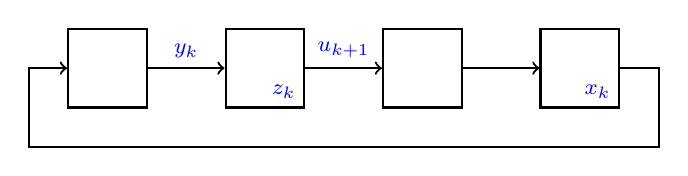
\begin{tikzpicture}
    % Blocks
    \node[draw, rectangle, minimum width = 1cm, minimum height = 1 cm, thick] (s) at (0,0) {$\sensor$};
    \node[draw, rectangle, minimum width = 1cm, minimum height = 1 cm, thick] (c) at (2,0) {$\ctrler$};
    \node[draw, rectangle, minimum width = 1cm, minimum height = 1 cm, thick] (a) at (4,0) {$\actuator$};
    \node[draw, rectangle, minimum width = 1cm, minimum height = 1 cm, thick] (p) at (6,0) {$\plant$};

    \node[anchor=south east, font=\footnotesize, blue] (z) at (c.south east) {$z_k$};
    \node[anchor=south east, font=\footnotesize, blue] (x) at (p.south east) {$x_k$};

    % Arrows
    \draw[->, thick] (s) -- node[above, blue, font=\footnotesize] {$y_k$} (c.west);
    \draw[->, thick] (c) -- node[above, blue, font=\footnotesize] {$u_{k+1}$} (a.west);
    \draw[->, thick] (a) -- (p.west);
    \draw[->, thick] (p.east) -| (7, -1) -| (-1, 0) -- (s.west);
\end{tikzpicture}
